\documentclass[class=beamer]{standalone}

\usetheme{technikum}
\usepackage{preamble}
\begin{document}
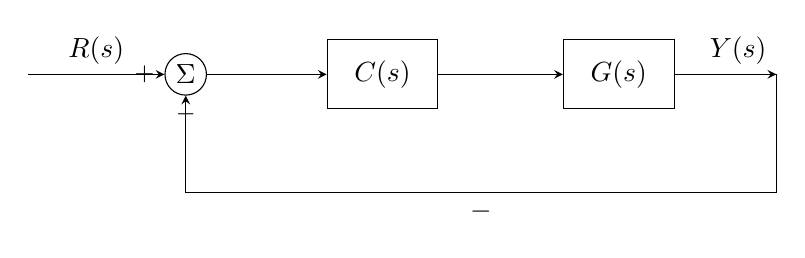
\begin{tikzpicture}[
    block/.style={rectangle, draw, minimum height=2.5em, minimum width=4em, align=center},
    sum/.style={circle, draw, minimum size=1.5em, inner sep=0pt},
    >=stealth
]
    % Blocks
    \node[sum]   (sum)        at (0,0)    {$\Sigma$};
    \node[block] (controller) at (2.5,0)  {$C(s)$};
    \node[block] (plant)      at (5.5,0)  {$G(s)$};

    % Input
    \draw[->] (-2,0) -- node[above] {$R(s)$} (sum);

    % Forward path
    \draw[->] (sum) -- (controller);
    \draw[->] (controller) -- (plant);

    % Output
    \draw[->] (plant) -- ++(2,0) node[above left] {$Y(s)$};

    % Feedback
    \coordinate (fb) at (7.5,0);
    \coordinate (fbdown) at (7.5,-1.5);
    \coordinate (fbleft) at (0,-1.5);

    \draw (plant.east) -- (fb);
    \draw[->] (fb) -- (fbdown) -- node[below] {$-$} (fbleft) -- (sum);

    % Signs at summing junction
    \node[left]  at (sum.west)  {\small $+$};
    \node[below] at (sum.south) {\small $-$};
\end{tikzpicture}
\end{document}
